\documentclass[11pt,]{article}
\usepackage[left=1in,top=1in,right=1in,bottom=1in]{geometry}
\newcommand*{\authorfont}{\fontfamily{phv}\selectfont}
\usepackage[]{mathpazo}


  \usepackage[T1]{fontenc}
  \usepackage[utf8]{inputenc}



\usepackage{abstract}
\renewcommand{\abstractname}{}    % clear the title
\renewcommand{\absnamepos}{empty} % originally center

\renewenvironment{abstract}
 {{%
    \setlength{\leftmargin}{0mm}
    \setlength{\rightmargin}{\leftmargin}%
  }%
  \relax}
 {\endlist}

\makeatletter
\def\@maketitle{%
  \newpage
%  \null
%  \vskip 2em%
%  \begin{center}%
  \let \footnote \thanks
    {\fontsize{18}{20}\selectfont\raggedright  \setlength{\parindent}{0pt} \@title \par}%
}
%\fi
\makeatother




\setcounter{secnumdepth}{0}

\usepackage{color}
\usepackage{fancyvrb}
\newcommand{\VerbBar}{|}
\newcommand{\VERB}{\Verb[commandchars=\\\{\}]}
\DefineVerbatimEnvironment{Highlighting}{Verbatim}{commandchars=\\\{\}}
% Add ',fontsize=\small' for more characters per line
\usepackage{framed}
\definecolor{shadecolor}{RGB}{248,248,248}
\newenvironment{Shaded}{\begin{snugshade}}{\end{snugshade}}
\newcommand{\KeywordTok}[1]{\textcolor[rgb]{0.13,0.29,0.53}{\textbf{{#1}}}}
\newcommand{\DataTypeTok}[1]{\textcolor[rgb]{0.13,0.29,0.53}{{#1}}}
\newcommand{\DecValTok}[1]{\textcolor[rgb]{0.00,0.00,0.81}{{#1}}}
\newcommand{\BaseNTok}[1]{\textcolor[rgb]{0.00,0.00,0.81}{{#1}}}
\newcommand{\FloatTok}[1]{\textcolor[rgb]{0.00,0.00,0.81}{{#1}}}
\newcommand{\ConstantTok}[1]{\textcolor[rgb]{0.00,0.00,0.00}{{#1}}}
\newcommand{\CharTok}[1]{\textcolor[rgb]{0.31,0.60,0.02}{{#1}}}
\newcommand{\SpecialCharTok}[1]{\textcolor[rgb]{0.00,0.00,0.00}{{#1}}}
\newcommand{\StringTok}[1]{\textcolor[rgb]{0.31,0.60,0.02}{{#1}}}
\newcommand{\VerbatimStringTok}[1]{\textcolor[rgb]{0.31,0.60,0.02}{{#1}}}
\newcommand{\SpecialStringTok}[1]{\textcolor[rgb]{0.31,0.60,0.02}{{#1}}}
\newcommand{\ImportTok}[1]{{#1}}
\newcommand{\CommentTok}[1]{\textcolor[rgb]{0.56,0.35,0.01}{\textit{{#1}}}}
\newcommand{\DocumentationTok}[1]{\textcolor[rgb]{0.56,0.35,0.01}{\textbf{\textit{{#1}}}}}
\newcommand{\AnnotationTok}[1]{\textcolor[rgb]{0.56,0.35,0.01}{\textbf{\textit{{#1}}}}}
\newcommand{\CommentVarTok}[1]{\textcolor[rgb]{0.56,0.35,0.01}{\textbf{\textit{{#1}}}}}
\newcommand{\OtherTok}[1]{\textcolor[rgb]{0.56,0.35,0.01}{{#1}}}
\newcommand{\FunctionTok}[1]{\textcolor[rgb]{0.00,0.00,0.00}{{#1}}}
\newcommand{\VariableTok}[1]{\textcolor[rgb]{0.00,0.00,0.00}{{#1}}}
\newcommand{\ControlFlowTok}[1]{\textcolor[rgb]{0.13,0.29,0.53}{\textbf{{#1}}}}
\newcommand{\OperatorTok}[1]{\textcolor[rgb]{0.81,0.36,0.00}{\textbf{{#1}}}}
\newcommand{\BuiltInTok}[1]{{#1}}
\newcommand{\ExtensionTok}[1]{{#1}}
\newcommand{\PreprocessorTok}[1]{\textcolor[rgb]{0.56,0.35,0.01}{\textit{{#1}}}}
\newcommand{\AttributeTok}[1]{\textcolor[rgb]{0.77,0.63,0.00}{{#1}}}
\newcommand{\RegionMarkerTok}[1]{{#1}}
\newcommand{\InformationTok}[1]{\textcolor[rgb]{0.56,0.35,0.01}{\textbf{\textit{{#1}}}}}
\newcommand{\WarningTok}[1]{\textcolor[rgb]{0.56,0.35,0.01}{\textbf{\textit{{#1}}}}}
\newcommand{\AlertTok}[1]{\textcolor[rgb]{0.94,0.16,0.16}{{#1}}}
\newcommand{\ErrorTok}[1]{\textcolor[rgb]{0.64,0.00,0.00}{\textbf{{#1}}}}
\newcommand{\NormalTok}[1]{{#1}}
\usepackage{longtable,booktabs}

\usepackage{graphicx,grffile}
\makeatletter
\def\maxwidth{\ifdim\Gin@nat@width>\linewidth\linewidth\else\Gin@nat@width\fi}
\def\maxheight{\ifdim\Gin@nat@height>\textheight\textheight\else\Gin@nat@height\fi}
\makeatother
% Scale images if necessary, so that they will not overflow the page
% margins by default, and it is still possible to overwrite the defaults
% using explicit options in \includegraphics[width, height, ...]{}
\setkeys{Gin}{width=\maxwidth,height=\maxheight,keepaspectratio}

\title{A demographic-based service-area toolkit \thanks{Replication files are available on the author's Github account
(\url{http://github.com/johnmbrandt}). \textbf{Current version}:
December 19, 2017; \textbf{Corresponding author}:
\href{mailto:john.brandt@yale.edu}{\nolinkurl{john.brandt@yale.edu}}.}  }



\author{\Large John M. Brandt\vspace{0.05in} \newline\normalsize\emph{Yale University}  }


\date{}

\usepackage{titlesec}

\titleformat*{\section}{\normalsize\bfseries}
\titleformat*{\subsection}{\normalsize\itshape}
\titleformat*{\subsubsection}{\normalsize\itshape}
\titleformat*{\paragraph}{\normalsize\itshape}
\titleformat*{\subparagraph}{\normalsize\itshape}


\usepackage{natbib}
\bibliographystyle{apsr}
\usepackage[strings]{underscore} % protect underscores in most circumstances



\newtheorem{hypothesis}{Hypothesis}
\usepackage{setspace}

\makeatletter
\@ifpackageloaded{hyperref}{}{%
\ifxetex
  \PassOptionsToPackage{hyphens}{url}\usepackage[setpagesize=false, % page size defined by xetex
              unicode=false, % unicode breaks when used with xetex
              xetex]{hyperref}
\else
  \PassOptionsToPackage{hyphens}{url}\usepackage[unicode=true]{hyperref}
\fi
}

\@ifpackageloaded{color}{
    \PassOptionsToPackage{usenames,dvipsnames}{color}
}{%
    \usepackage[usenames,dvipsnames]{color}
}
\makeatother
\hypersetup{breaklinks=true,
            bookmarks=true,
            pdfauthor={John M. Brandt (Yale University)},
             pdfkeywords = {},  
            pdftitle={A demographic-based service-area toolkit},
            colorlinks=true,
            citecolor=blue,
            urlcolor=blue,
            linkcolor=magenta,
            pdfborder={0 0 0}}
\urlstyle{same}  % don't use monospace font for urls

% set default figure placement to htbp
\makeatletter
\def\fps@figure{htbp}
\makeatother



% add tightlist ----------
\providecommand{\tightlist}{%
\setlength{\itemsep}{0pt}\setlength{\parskip}{0pt}}

\begin{document}
	
% \pagenumbering{arabic}% resets `page` counter to 1 
%
% \maketitle

{% \usefont{T1}{pnc}{m}{n}
\setlength{\parindent}{0pt}
\thispagestyle{plain}
{\fontsize{18}{20}\selectfont\raggedright 
\maketitle  % title \par  

}

{
   \vskip 13.5pt\relax \normalsize\fontsize{11}{12} 
\textbf{\authorfont John M. Brandt} \hskip 15pt \emph{\small Yale University}   

}

}








\begin{abstract}

    \hbox{\vrule height .2pt width 39.14pc}

    \vskip 8.5pt % \small 

\noindent Transportation distance is a primary indicator of the population served
by a given location. For instance, most people would probably drive 5
miles to get to a park or mental health clinic, but many less would
choose to drive 50 miles. While some locations, like salons or retail
stores, may want to target specific populations, other locations, like
WIC centers, hospitals, or parks, aim to serve all populations equally.
This toolkit provides an easy means with which to identify groups of
people that are better or worse served by any given facility. Using
census data, road network data, and the locations of facilities, the
toolkit calculates, per county, the percentage of a given demographic
within a user-specified driving time or distance from a facility
location. The example included in this report calculates the
county-by-county access of the total population, black residents, and
single mothers to WIC centers in New York. However, this toolkit can
calculate the served demographics of any facility type, with any amount
of distance, and with respect to any census data (race, income,
household type, education, or age). For instance, one could determine
whether a youth fashion brand is properly targeting youth, or whether
hospitals are properly located near elderly people. Calculating these
service percentiles by county allows decision makers to easily identify
regions where improvement is needed.


    \hbox{\vrule height .2pt width 39.14pc}


\end{abstract}


\vskip 6.5pt


\noindent  \section{Introduction}\label{introduction}

The workflow for this script is broken down into three parts, each a
separate ArcToolbox script:

\begin{itemize}
\tightlist
\item
  Creating the service area-layer
\item
  Calculating the percent-coverage of each census block
\item
  Calculating the percent-coverage for a given demographic aggregated to
  a larger census level
\end{itemize}

\noindent The first part uses a
\href{https://www.arcgis.com/home/item.html?id=0f4ae38e76b241609057286f6b34f597}{network
dataset} and the locations of facilities, along with a user-specified
service area (in distance or time), to generate a shapefile of the areas
served. \vspace{3mm}

\noindent The second part uses
\href{https://www.census.gov/geo/maps-data/data/tiger-data.html}{census
block group} geometry to calculate the area of the service area within
each census block, as well as the area of each census block. These two
variables are used to calculate the percentage of each census block that
is within the specified distance of a facility. \vspace{3mm}

\noindent The third part calculates the percentage of residents of a
specified demographic variable within each county in a region that are
serviced by a facility. Any census data variable can be used, including
race, income, household type, education, and age. \vspace{3mm}

\noindent The example included in this report calculates the
county-by-county access of the total population, black residents, and
single mothers to \href{http://www.nyskwic.org/map/kwicmap.cfm}{WIC
centers in New York.}

\begin{figure}[htbp]
\centering
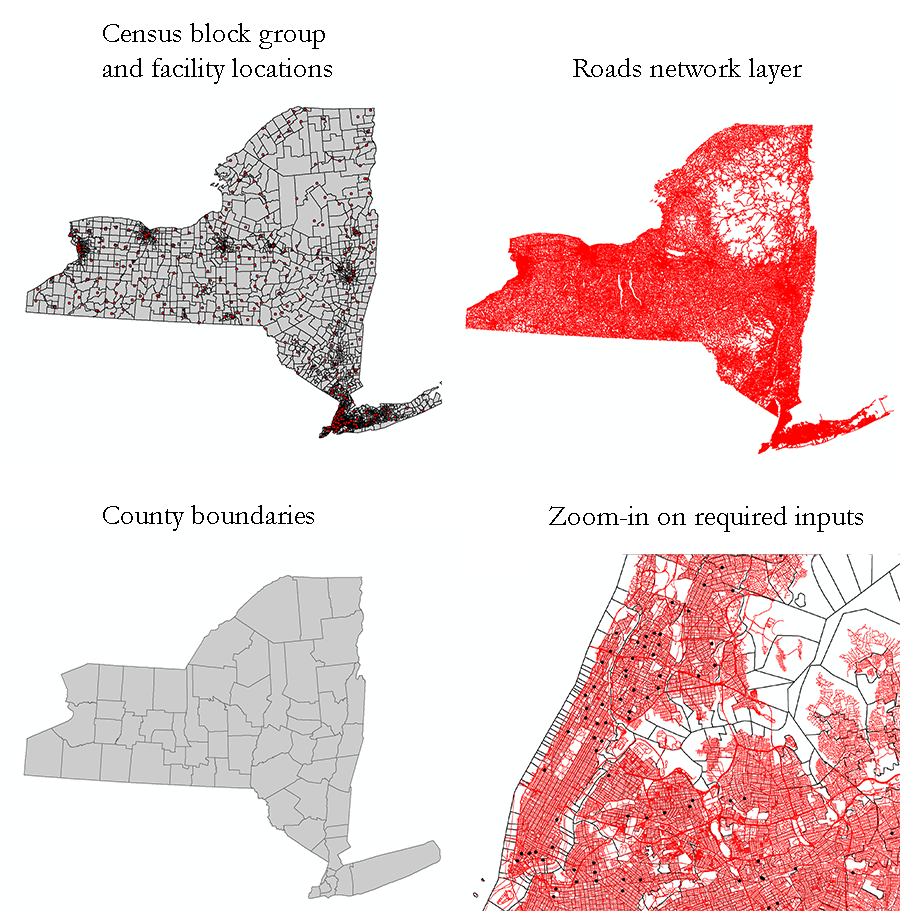
\includegraphics{/Users/johnbrandt/Google Drive/Yale/Semester 1/Environmental Regression/Final/inputs_2.png}
\caption{Required inputs}
\end{figure}

\section{Part 1 - Network
Calculations}\label{part-1---network-calculations}

\subsection{Inputs}\label{inputs}

This script takes the following inputs, in addition to requiring the
Network Analyst and Spatial Analyst ArcGIS extensions.

\begin{longtable}[]{@{}ll@{}}
\toprule
Input & Description\tabularnewline
\midrule
\endhead
NetworkRoad & Network layer of roads\tabularnewline
Facility & Feature class containing point location of
facilities\tabularnewline
ServiceAreaRadius & How many feet to calculate service
area\tabularnewline
CensusLayer & Feature class of census block group data\tabularnewline
DissolveField & Census layer object ID field\tabularnewline
\tabularnewline
outLayerFile & Name of service area layer (.shp)\tabularnewline
outputDissolved & Dissolved surface area layer (.shp)\tabularnewline
outputJoined & Final output layer (.shp)\tabularnewline
\bottomrule
\end{longtable}

\subsection{Code}\label{code}

\noindent Full code is available
\href{https://github.com/johnmbrandt/public-resource-mapper}{online}.
Begin by importing the required modules, turning the required extensions
on, and setting the input and output files and variables. Upon success,
we log a message to the console notifying the user that the script is
continuing.

\begin{Shaded}
\begin{Highlighting}[]
\CommentTok{#Import system modules}
\ImportTok{import} \NormalTok{sys, os, math, shutil, arcpy, string, traceback}
\ImportTok{from} \NormalTok{arcpy }\ImportTok{import} \NormalTok{env}
\ImportTok{from} \NormalTok{arcpy.sa }\ImportTok{import} \OperatorTok{*}


\ControlFlowTok{try}\NormalTok{:}
    \CommentTok{# Check out the necessary extensions}
    \NormalTok{arcpy.CheckOutExtension(}\StringTok{"Network"}\NormalTok{)}
    \NormalTok{arcpy.CheckOutExtension(}\StringTok{"Spatial"}\NormalTok{)}

    \CommentTok{# Set environment & output settings}
    \NormalTok{env.overwriteOutput }\OperatorTok{=} \VariableTok{True}

    \CommentTok{# Set input variables}
    \NormalTok{NetworkRoad }\OperatorTok{=} \NormalTok{arcpy.GetParameterAsText(}\DecValTok{0}\NormalTok{)        }\CommentTok{# Network dataset (.lyr)}
    \NormalTok{Facility }\OperatorTok{=} \NormalTok{arcpy.GetParameterAsText(}\DecValTok{1}\NormalTok{)           }\CommentTok{# Facility locations}
    \NormalTok{ServiceAreaRadius }\OperatorTok{=} \NormalTok{arcpy.GetParameterAsText(}\DecValTok{2}\NormalTok{)  }\CommentTok{# Service area radius (feet)}
    \NormalTok{CensusLayer }\OperatorTok{=} \NormalTok{arcpy.GetParameterAsText(}\DecValTok{3}\NormalTok{)        }\CommentTok{# Census tracts layer (.shp)}
    \NormalTok{DissolveField }\OperatorTok{=} \NormalTok{arcpy.GetParameterAsText(}\DecValTok{4}\NormalTok{)      }\CommentTok{# Identifier in census layer}

    \CommentTok{# Set output variables}
    \NormalTok{outLayerFile }\OperatorTok{=} \NormalTok{arcpy.GetParameterAsText(}\DecValTok{5}\NormalTok{)}
    \NormalTok{outputDissolved }\OperatorTok{=} \NormalTok{arcpy.GetParameterAsText(}\DecValTok{6}\NormalTok{)}
    \NormalTok{outputJoined }\OperatorTok{=} \NormalTok{arcpy.GetParameterAsText(}\DecValTok{7}\NormalTok{)}
    
    \NormalTok{arcpy.AddMessage(}\StringTok{'}\CharTok{\textbackslash{}n}\StringTok{'} \OperatorTok{+} \StringTok{"The network road input shapefile name is: "}
      \OperatorTok{+}\NormalTok{NetworkRoad}\OperatorTok{+}\StringTok{'}\CharTok{\textbackslash{}n}\StringTok{'}\NormalTok{)}
\end{Highlighting}
\end{Shaded}

\noindent Next, the network dataset is built from the input network
layer, to which an empty service area layer is appended. Facility
locations are added to the network layer, which is then solved. This
results in a .lyr output with the polygonal service areas as a sublayer.

\begin{Shaded}
\begin{Highlighting}[]

    \CommentTok{# Build the network dataset}
    \NormalTok{arcpy.na.BuildNetwork(in_network_dataset}\OperatorTok{=}\NormalTok{NetworkRoad)}
    \NormalTok{arcpy.AddMessage(}\StringTok{'}\CharTok{\textbackslash{}n}\StringTok{'} \OperatorTok{+} \StringTok{"Network dataset finished"}\NormalTok{)}

    \CommentTok{# Create a service area layer}
    \NormalTok{outLayerName }\OperatorTok{=} \NormalTok{arcpy.na.MakeServiceAreaLayer(in_network_dataset}\OperatorTok{=}\NormalTok{NetworkRoad,}
                                \NormalTok{impedance_attribute}\OperatorTok{=}\StringTok{"Length"}\NormalTok{,}
                                \NormalTok{travel_from_to}\OperatorTok{=}\StringTok{"TRAVEL_FROM"}\NormalTok{,}
                                \NormalTok{default_break_values}\OperatorTok{=}\NormalTok{ServiceAreaRadius,}
                                \NormalTok{polygon_type}\OperatorTok{=}\StringTok{"SIMPLE_POLYS"}\NormalTok{,}
                                \NormalTok{merge}\OperatorTok{=}\StringTok{"NO_MERGE"}\NormalTok{,}
                                \NormalTok{nesting_type}\OperatorTok{=}\StringTok{"RINGS"}\NormalTok{,}
                                \NormalTok{line_type}\OperatorTok{=}\StringTok{"NO_LINES"}\NormalTok{,}
                                \NormalTok{overlap}\OperatorTok{=}\StringTok{"OVERLAP"}\NormalTok{,}
                                \NormalTok{split}\OperatorTok{=}\StringTok{"NO_SPLIT"}\NormalTok{,}
                                \NormalTok{excluded_source_name}\OperatorTok{=}\StringTok{""}\NormalTok{,}
                                \NormalTok{accumulate_attribute_name}\OperatorTok{=}\StringTok{""}\NormalTok{,}
                                \NormalTok{UTurn_policy}\OperatorTok{=}\StringTok{"ALLOW_UTURNS"}\NormalTok{,}
                                \NormalTok{restriction_attribute_name}\OperatorTok{=}\StringTok{"Oneway"}\NormalTok{,}
                                \NormalTok{polygon_trim}\OperatorTok{=}\StringTok{"TRIM_POLYS"}\NormalTok{,}
                                \NormalTok{poly_trim_value}\OperatorTok{=}\StringTok{"250 Meters"}\NormalTok{,}
                                \NormalTok{lines_source_fields}\OperatorTok{=}\StringTok{"NO_LINES_SOURCE_FIELDS"}\NormalTok{,}
                                \NormalTok{hierarchy}\OperatorTok{=}\StringTok{"NO_HIERARCHY"}\NormalTok{, time_of_day}\OperatorTok{=}\StringTok{""}\NormalTok{)}

    \CommentTok{# Get the output of the service layer}
    \NormalTok{FacilitiesInterim }\OperatorTok{=} \NormalTok{outLayerName.getOutput(}\DecValTok{0}\NormalTok{)}

    \CommentTok{# Create a variable referencing the list of sublayers of the service area layer}
    \NormalTok{naClasses }\OperatorTok{=} \NormalTok{arcpy.na.GetNAClassNames(FacilitiesInterim)}

    \CommentTok{# Create a variable storing the name of the sublayer containing the facilities}
    \NormalTok{FacilitiesLayer }\OperatorTok{=} \NormalTok{arcpy.na.GetNAClassNames(FacilitiesInterim)[}\StringTok{"Facilities"}\NormalTok{]}

    \CommentTok{# Add the shapefile of locations to the service area layer}
    \NormalTok{arcpy.na.AddLocations(outLayerName, FacilitiesLayer, Facility, }\StringTok{""}\NormalTok{, }\StringTok{""}\NormalTok{)}

    \CommentTok{# Solve the service area}
    \NormalTok{arcpy.na.Solve(outLayerName)}
\end{Highlighting}
\end{Shaded}

\noindent In order to do calculations based upon the polygonal area, we
must extract the sublayer. To do this, we make use of the arcpy mapping
function on the \texttt{FacilitiesInterim} object, which contains the
output of the service area layer. We use the \texttt{naClasses} variable
defined above, containing the names of the sublayers, to extract data
from the \texttt{SAPolygons} sublayer. This layer is copied and saved as
a shapefile to the user-specified location.

\begin{Shaded}
\begin{Highlighting}[]

    \CommentTok{# Use arcpy mapping and the naClasses variable we defined above to create}
    \CommentTok{# a variable storing the polygons sublayer}
    \NormalTok{polygonsSubLayer }\OperatorTok{=} \NormalTok{arcpy.mapping.ListLayers(FacilitiesInterim,}
      \NormalTok{naClasses[}\StringTok{"SAPolygons"}\NormalTok{])[}\DecValTok{0}\NormalTok{]}

    \CommentTok{# Copy the polygons sublayer to the disk, as a shapefile}
    \NormalTok{arcpy.CopyFeatures_management(polygonsSubLayer, outLayerFile)}
\end{Highlighting}
\end{Shaded}

\noindent The feature class containing service area polygons has regions
of overlap that are served by multiple facilities. The borders of these
polygons are dissolved to create a continuous polygon of the service
area. This shapefile is also saved to the disk.

\begin{Shaded}
\begin{Highlighting}[]

    \CommentTok{# Dissolve the borders between service areas within each census polygon}
    \NormalTok{dissolved }\OperatorTok{=} \NormalTok{arcpy.Dissolve_management(in_features}\OperatorTok{=}\NormalTok{outLayerFile,}
                                       \NormalTok{dissolve_field}\OperatorTok{=}\StringTok{"FromBreak"}\NormalTok{,}
                                       \NormalTok{statistics_fields}\OperatorTok{=}\StringTok{""}\NormalTok{,}
                                       \NormalTok{multi_part}\OperatorTok{=}\StringTok{"MULTI_PART"}\NormalTok{,}
                                       \NormalTok{unsplit_lines}\OperatorTok{=}\StringTok{"DISSOLVE_LINES"}\NormalTok{)}

    \CommentTok{# Export the dissolved shapefile to the disk}
    \NormalTok{arcpy.CopyFeatures_management(dissolved, outputDissolved)}
\end{Highlighting}
\end{Shaded}

\noindent Next, the dissolved service area is intersected with the
census block group data. The area of each polygon (representing the
service area of each census block group) is calculated, as is the area
of the census block group itself. Finally, we join these two layers to
create one output shapefile containing block-group census data as well
as a field of the serviced area and a field of the total area.

\begin{Shaded}
\begin{Highlighting}[]
    \CommentTok{# Calculate the intersection between the service area and the census layer}
    \NormalTok{intersected }\OperatorTok{=} \NormalTok{arcpy.Intersect_analysis([dissolved, CensusLayer],}
                                           \NormalTok{join_attributes}\OperatorTok{=}\StringTok{"ALL"}\NormalTok{,}
                                           \NormalTok{cluster_tolerance}\OperatorTok{=}\StringTok{"-1 Unknown"}\NormalTok{,}
                                           \NormalTok{output_type}\OperatorTok{=}\StringTok{"INPUT"}\NormalTok{)}

    \CommentTok{# Calculate the area of the dissolved polygons within each census polygon}
    \NormalTok{intersected_area }\OperatorTok{=} \NormalTok{arcpy.AddGeometryAttributes_management(}
                                            \NormalTok{Input_Features }\OperatorTok{=} \NormalTok{intersected,}
                                            \NormalTok{Geometry_Properties}\OperatorTok{=}\StringTok{"AREA_GEODESIC"}\NormalTok{,}
                                            \NormalTok{Length_Unit}\OperatorTok{=}\StringTok{""}\NormalTok{,}
                                            \NormalTok{Area_Unit}\OperatorTok{=}\StringTok{"SQUARE_MILES_US"}\NormalTok{,}
                                            \NormalTok{Coordinate_System}\OperatorTok{=}\StringTok{""}\NormalTok{)}

    \CommentTok{# Calculate the area of each census polygon}
    \NormalTok{Census_area }\OperatorTok{=} \NormalTok{arcpy.AddGeometryAttributes_management(}
                                            \NormalTok{Input_Features }\OperatorTok{=} \NormalTok{CensusLayer,}
                                            \NormalTok{Geometry_Properties}\OperatorTok{=}\StringTok{"AREA_GEODESIC"}\NormalTok{,}
                                                        \NormalTok{Length_Unit}\OperatorTok{=}\StringTok{""}\NormalTok{,}
                                                        \NormalTok{Area_Unit}\OperatorTok{=}\StringTok{"SQUARE_MILES_US"}\NormalTok{,}
                                                        \NormalTok{Coordinate_System}\OperatorTok{=}\StringTok{""}\NormalTok{)}

    \CommentTok{# Join the layer of the area of the dissolved polygons to the census layer}
    \NormalTok{arcpy.SpatialJoin_analysis(target_features}\OperatorTok{=}\NormalTok{Census_area,}
                        \NormalTok{join_features}\OperatorTok{=}\NormalTok{intersected_area,}
                        \NormalTok{out_feature_class }\OperatorTok{=} \NormalTok{outputJoined,}
                        \NormalTok{join_operation}\OperatorTok{=}\StringTok{"JOIN_ONE_TO_ONE"}\NormalTok{,}
                        \NormalTok{join_type}\OperatorTok{=}\StringTok{"KEEP_ALL"}\NormalTok{,}
                        \NormalTok{match_option}\OperatorTok{=}\StringTok{"CONTAINS"}\NormalTok{,}
                        \NormalTok{search_radius}\OperatorTok{=}\StringTok{""}\NormalTok{,}
                        \NormalTok{distance_field_name}\OperatorTok{=}\StringTok{""}\NormalTok{)}

    \CommentTok{# When done, turn off the Spatial Analysis and Network Analysis Extensions}
    \NormalTok{arcpy.CheckInExtension(}\StringTok{"Network"}\NormalTok{)}
    \NormalTok{arcpy.CheckInExtension(}\StringTok{"Spatial"}\NormalTok{)}
\end{Highlighting}
\end{Shaded}

\noindent Report an error message to the arcToolbox script window if the
script fails to execute.

\begin{Shaded}
\begin{Highlighting}[]
\ControlFlowTok{except} \PreprocessorTok{Exception} \ImportTok{as} \NormalTok{e:}
    \NormalTok{arcpy.AddError(}\StringTok{'}\CharTok{\textbackslash{}n}\StringTok{'} \OperatorTok{+} \StringTok{"Script failed because: }\CharTok{\textbackslash{}t\textbackslash{}t}\StringTok{"} \OperatorTok{+} \NormalTok{e.message )}
    \NormalTok{exceptionreport }\OperatorTok{=} \NormalTok{sys.exc_info()[}\DecValTok{2}\NormalTok{]}
    \NormalTok{arcpy.AddError(}\StringTok{"at this location: }\CharTok{\textbackslash{}n\textbackslash{}n}\StringTok{"} \OperatorTok{+}
    \NormalTok{traceback.format_tb(exceptionreport)[}\DecValTok{0}\NormalTok{]}\OperatorTok{+} \StringTok{"}\CharTok{\textbackslash{}n}\StringTok{"}\NormalTok{)}
\end{Highlighting}
\end{Shaded}

\begin{figure}[htbp]
\centering
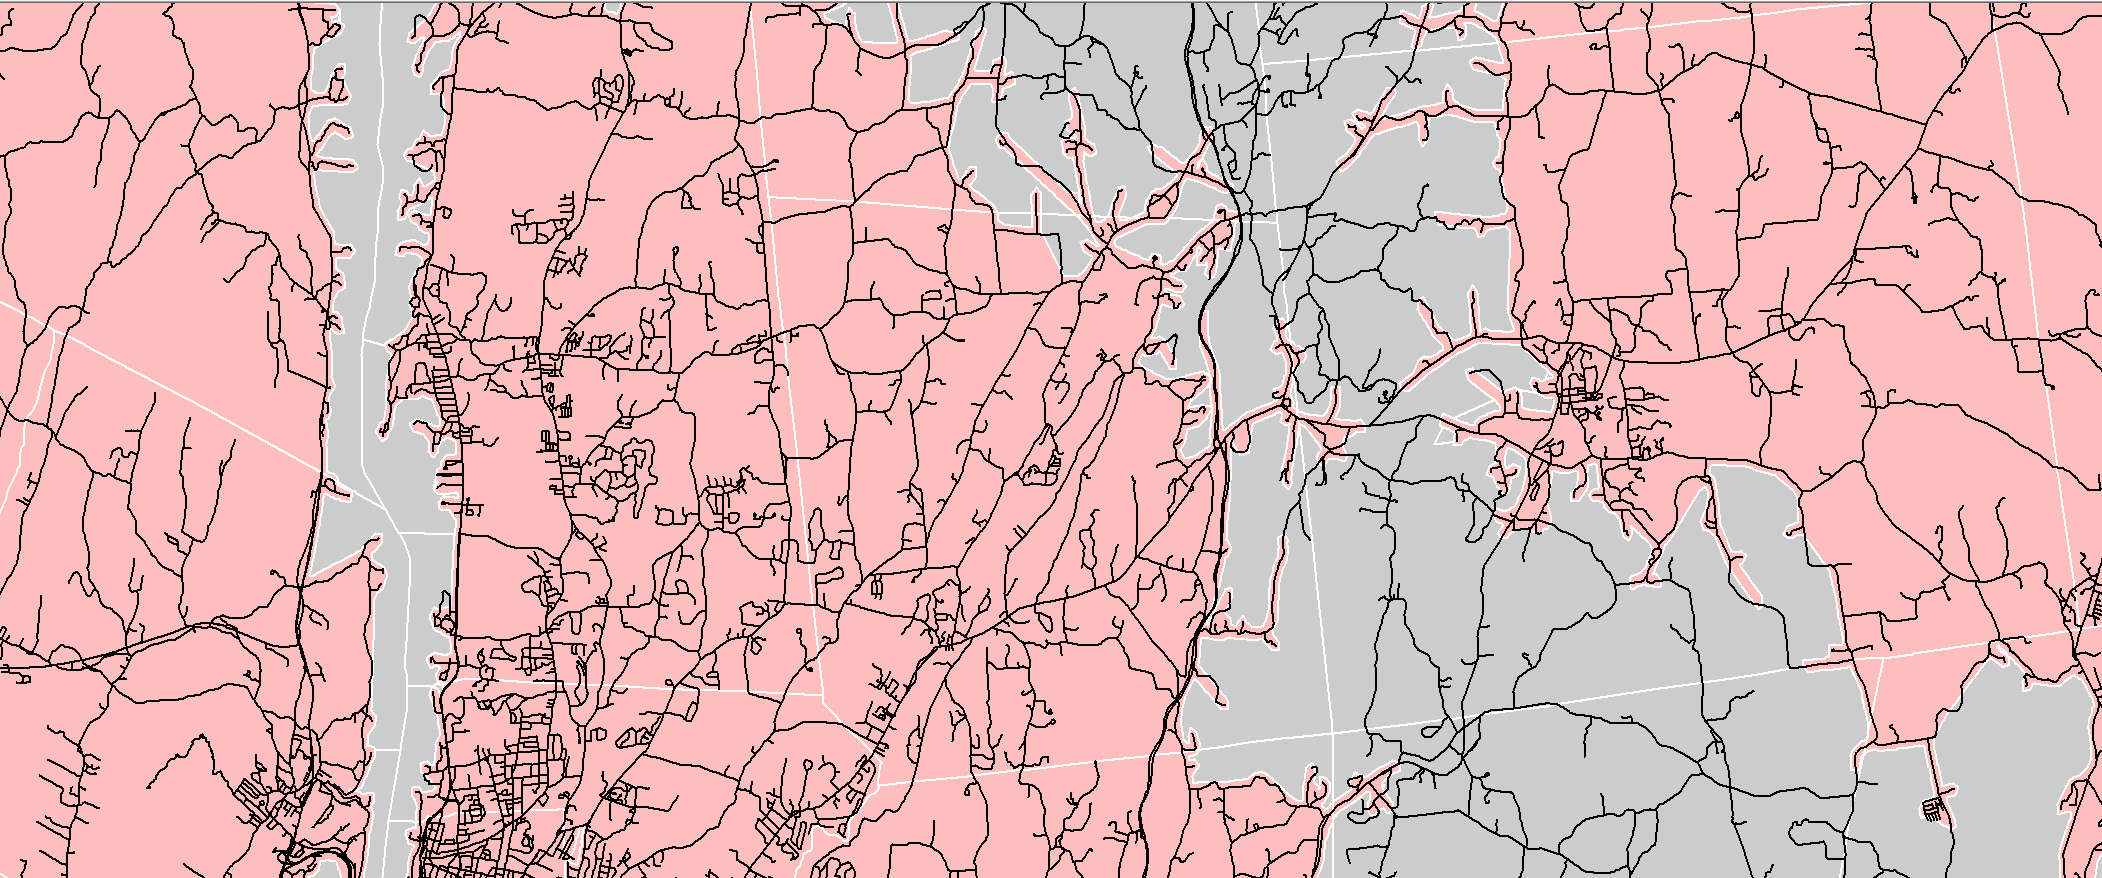
\includegraphics{/Users/johnbrandt/Google Drive/Yale/Semester 1/Environmental Regression/Final/part_1_zoom_in_2.png}
\caption{Part 1 output, showing regions within (pink) and outside (grey)
the service area.}
\end{figure}

\pagebreak

\section{Part 2 - Percent serviced
area}\label{part-2---percent-serviced-area}

\subsection{Inputs}\label{inputs-1}

This script takes the following inputs and outputs:

\begin{longtable}[]{@{}ll@{}}
\toprule
\begin{minipage}[b]{0.19\columnwidth}\raggedright\strut
Input\strut
\end{minipage} & \begin{minipage}[b]{0.75\columnwidth}\raggedright\strut
Description\strut
\end{minipage}\tabularnewline
\midrule
\endhead
\begin{minipage}[t]{0.19\columnwidth}\raggedright\strut
input\_shapefile\strut
\end{minipage} & \begin{minipage}[t]{0.75\columnwidth}\raggedright\strut
Output of Part 1, with areas of service per census block group\strut
\end{minipage}\tabularnewline
\begin{minipage}[t]{0.19\columnwidth}\raggedright\strut
service\_area\strut
\end{minipage} & \begin{minipage}[t]{0.75\columnwidth}\raggedright\strut
Field within input\_shapefile, areas of service polygons\strut
\end{minipage}\tabularnewline
\begin{minipage}[t]{0.19\columnwidth}\raggedright\strut
census\_area\strut
\end{minipage} & \begin{minipage}[t]{0.75\columnwidth}\raggedright\strut
Field within input\_shapefile, areas of census block polygons\strut
\end{minipage}\tabularnewline
\begin{minipage}[t]{0.19\columnwidth}\raggedright\strut
\strut
\end{minipage}\tabularnewline
\begin{minipage}[t]{0.19\columnwidth}\raggedright\strut
output\_field\strut
\end{minipage} & \begin{minipage}[t]{0.75\columnwidth}\raggedright\strut
Field to be calculated in output\_shapefile, percent serviced area\strut
\end{minipage}\tabularnewline
\begin{minipage}[t]{0.19\columnwidth}\raggedright\strut
output\_shapefile\strut
\end{minipage} & \begin{minipage}[t]{0.75\columnwidth}\raggedright\strut
Location of output shapefile\strut
\end{minipage}\tabularnewline
\bottomrule
\end{longtable}

\subsection{Code}\label{code-1}

\noindent Begin by importing the required modules and setting the input
and output files and variables.

\begin{Shaded}
\begin{Highlighting}[]
\CommentTok{#Import system modules}
\ImportTok{import} \NormalTok{sys, os, math, shutil, arcpy, string, traceback}
\NormalTok{arcpy.env.overwriteOutput }\OperatorTok{=} \VariableTok{True}

\ControlFlowTok{try}\NormalTok{:}

    \CommentTok{# Set input variables}
    \NormalTok{input_shapefile }\OperatorTok{=} \NormalTok{arcpy.GetParameterAsText(}\DecValTok{0}\NormalTok{)   }
    \NormalTok{service_area }\OperatorTok{=} \NormalTok{arcpy.GetParameterAsText(}\DecValTok{1}\NormalTok{)}
    \NormalTok{census_area }\OperatorTok{=} \NormalTok{arcpy.GetParameterAsText(}\DecValTok{2}\NormalTok{)}

    \NormalTok{arcpy.AddMessage(}\StringTok{'}\CharTok{\textbackslash{}n}\StringTok{'} \OperatorTok{+} \StringTok{"The input shapefile is"} \OperatorTok{+} \NormalTok{input_shapefile }\OperatorTok{+} \StringTok{", and"}
        \OperatorTok{+} \NormalTok{service_area }\OperatorTok{+}  \StringTok{" and "} \OperatorTok{+} \NormalTok{census_area }\OperatorTok{+} \StringTok{"are the input fields."}\NormalTok{)}
    
    \CommentTok{# Set output variables}
    \NormalTok{output_field }\OperatorTok{=} \NormalTok{arcpy.GetParameterAsText(}\DecValTok{3}\NormalTok{)}
    \NormalTok{output_shapefile }\OperatorTok{=} \NormalTok{arcpy.GetParameterAsText(}\DecValTok{4}\NormalTok{)}

    \NormalTok{arcpy.AddMessage(}\StringTok{"The name of the field to be added is "} \OperatorTok{+} \NormalTok{output_field }\OperatorTok{+} \StringTok{"}\CharTok{\textbackslash{}n}\StringTok{"}\NormalTok{)}
    \NormalTok{arcpy.AddMessage(}\StringTok{'}\CharTok{\textbackslash{}n}\StringTok{'} \OperatorTok{+} \StringTok{"The output shapefile is"} \OperatorTok{+} \NormalTok{output_shapefile)}
\end{Highlighting}
\end{Shaded}

\noindent The input is copied to a new shapefile which will be edited.
First, we add a new field to the shapefile that will hold the output
data. In order to iterate through each row, we create an
\texttt{UpdateCursor} object, called \texttt{ShpRecords}.

\begin{Shaded}
\begin{Highlighting}[]

    \CommentTok{# Create a new copy of the shapefile and save it as the output shapefile}
    \NormalTok{arcpy.Copy_management(input_shapefile, output_shapefile)}
    \NormalTok{arcpy.AddMessage(}\StringTok{'}\CharTok{\textbackslash{}n}\StringTok{'} \OperatorTok{+} \StringTok{"Copied"}\NormalTok{)}

    \CommentTok{# Add a new field to the output shapefile}
    \NormalTok{arcpy.AddField_management(output_shapefile, output_field, }\StringTok{"DOUBLE"}\NormalTok{, }\DecValTok{20}\NormalTok{, }\DecValTok{5}\NormalTok{)}
    \NormalTok{arcpy.AddMessage(}\StringTok{'}\CharTok{\textbackslash{}n}\StringTok{'} \OperatorTok{+} \StringTok{"New Field Added"}\NormalTok{)}

    \CommentTok{# Create a list of iterable records within the output shapefile}
    \NormalTok{ShpRecords }\OperatorTok{=} \NormalTok{arcpy.UpdateCursor(output_shapefile)}
    \NormalTok{arcpy.AddMessage(}\StringTok{'}\CharTok{\textbackslash{}n}\StringTok{'} \OperatorTok{+} \StringTok{"List made"}\NormalTok{)}
\end{Highlighting}
\end{Shaded}

\noindent By iterating over each record in the \texttt{ShpRecords}, we
calculate the percent of area within each census block group that is
within the service area of a facility. Specifically,
\texttt{service\_value} obtains the value of the area of the serviced
region, and \texttt{census\_value} obtains the value of the area of the
census block group. Dividing the former by the latter results in the
percent serviced area, which is saved to the output field defined in the
input section.

\begin{Shaded}
\begin{Highlighting}[]
    \CommentTok{# Iterate over each index in the shapefile}
    \ControlFlowTok{for} \NormalTok{record }\OperatorTok{in} \NormalTok{ShpRecords:}
        \NormalTok{service_value }\OperatorTok{=} \NormalTok{record.getValue(service_area)}
        \NormalTok{census_value }\OperatorTok{=} \NormalTok{record.getValue(census_area)}
        \NormalTok{result }\OperatorTok{=} \NormalTok{service_value}\OperatorTok{/}\NormalTok{census_value}
        \NormalTok{record.setValue(output_field, result)}
        \NormalTok{ShpRecords.updateRow(record)}

    \CommentTok{# Delete extraneous temp files}
    \KeywordTok{del} \NormalTok{ShpRecords}
    \KeywordTok{del} \NormalTok{record}
    
\ControlFlowTok{except} \PreprocessorTok{Exception} \ImportTok{as} \NormalTok{e:}
    \NormalTok{arcpy.AddError(}\StringTok{'}\CharTok{\textbackslash{}n}\StringTok{'} \OperatorTok{+} \StringTok{"Script failed because: }\CharTok{\textbackslash{}t\textbackslash{}t}\StringTok{"} \OperatorTok{+} \NormalTok{e.message )}
    \NormalTok{exceptionreport }\OperatorTok{=} \NormalTok{sys.exc_info()[}\DecValTok{2}\NormalTok{]}
    \NormalTok{arcpy.AddError(}\StringTok{"at this location: }\CharTok{\textbackslash{}n\textbackslash{}n}\StringTok{"} \OperatorTok{+} 
    \NormalTok{traceback.format_tb(exceptionreport)[}\DecValTok{0}\NormalTok{]}\OperatorTok{+} \StringTok{"}\CharTok{\textbackslash{}n}\StringTok{"}\NormalTok{)}
\end{Highlighting}
\end{Shaded}

\begin{figure}[htbp]
\centering
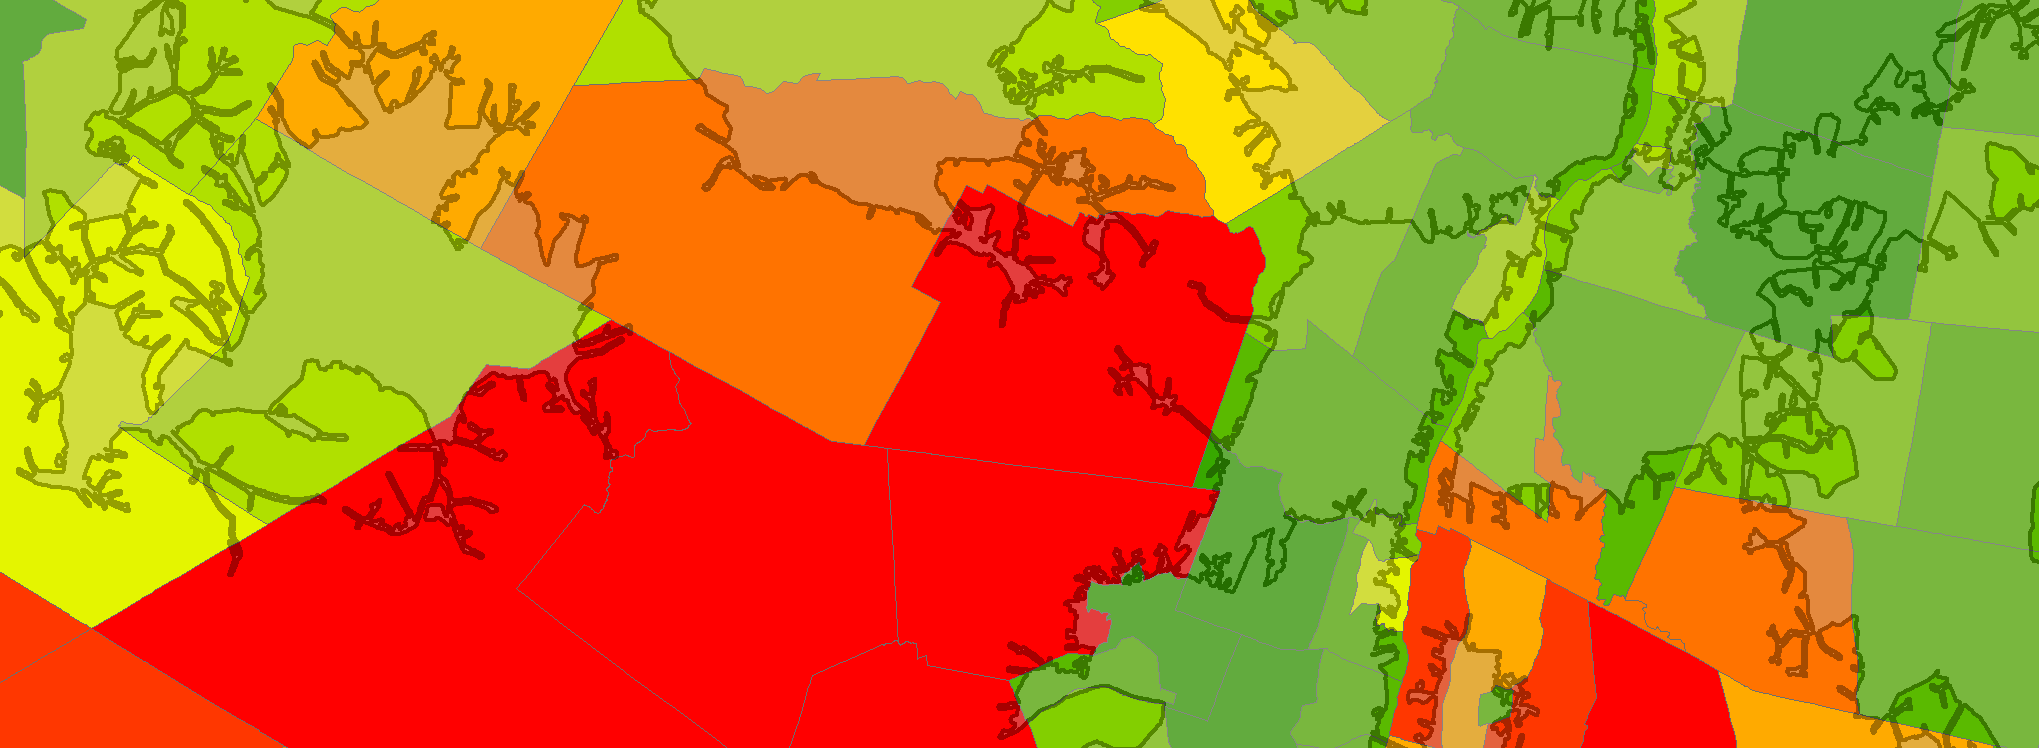
\includegraphics{/Users/johnbrandt/Google Drive/Yale/Semester 1/Environmental Regression/Final/part_2_zoom_in_2.png}
\caption{Part 2 output, showing block groups with high (green) and low
(red) service coverage.}
\end{figure}

\pagebreak

\section{Part 3 - Census
calculations}\label{part-3---census-calculations}

\subsection{Inputs}\label{inputs-2}

This script takes the following inputs:

\begin{longtable}[]{@{}ll@{}}
\toprule
\begin{minipage}[b]{0.23\columnwidth}\raggedright\strut
Input\strut
\end{minipage} & \begin{minipage}[b]{0.71\columnwidth}\raggedright\strut
Description\strut
\end{minipage}\tabularnewline
\midrule
\endhead
\begin{minipage}[t]{0.23\columnwidth}\raggedright\strut
input\_part\_2\strut
\end{minipage} & \begin{minipage}[t]{0.71\columnwidth}\raggedright\strut
Output of Part 2, percent coverage of service area by block group\strut
\end{minipage}\tabularnewline
\begin{minipage}[t]{0.23\columnwidth}\raggedright\strut
input\_census\_file\strut
\end{minipage} & \begin{minipage}[t]{0.71\columnwidth}\raggedright\strut
Feature class containing county boundaries\strut
\end{minipage}\tabularnewline
\begin{minipage}[t]{0.23\columnwidth}\raggedright\strut
\strut
\end{minipage}\tabularnewline
\begin{minipage}[t]{0.23\columnwidth}\raggedright\strut
percent\_coverage\strut
\end{minipage} & \begin{minipage}[t]{0.71\columnwidth}\raggedright\strut
Field within input\_part\_2, percent coverage of service area\strut
\end{minipage}\tabularnewline
\begin{minipage}[t]{0.23\columnwidth}\raggedright\strut
census\_input\_field\strut
\end{minipage} & \begin{minipage}[t]{0.71\columnwidth}\raggedright\strut
User-specified field in input\_part\_2, containing demographic
data\strut
\end{minipage}\tabularnewline
\begin{minipage}[t]{0.23\columnwidth}\raggedright\strut
dissolve\_field\strut
\end{minipage} & \begin{minipage}[t]{0.71\columnwidth}\raggedright\strut
Unique identifier within input\_census\_file to dissolve on\strut
\end{minipage}\tabularnewline
\begin{minipage}[t]{0.23\columnwidth}\raggedright\strut
\strut
\end{minipage}\tabularnewline
\begin{minipage}[t]{0.23\columnwidth}\raggedright\strut
total\_serve\_output\strut
\end{minipage} & \begin{minipage}[t]{0.71\columnwidth}\raggedright\strut
Output field, total number of demographic within county service
area\strut
\end{minipage}\tabularnewline
\begin{minipage}[t]{0.23\columnwidth}\raggedright\strut
percent\_serve\_output\strut
\end{minipage} & \begin{minipage}[t]{0.71\columnwidth}\raggedright\strut
Output field, percentage of county residents in service area\strut
\end{minipage}\tabularnewline
\begin{minipage}[t]{0.23\columnwidth}\raggedright\strut
\strut
\end{minipage}\tabularnewline
\begin{minipage}[t]{0.23\columnwidth}\raggedright\strut
output\_shapefile\strut
\end{minipage} & \begin{minipage}[t]{0.71\columnwidth}\raggedright\strut
Location of output shapefile\strut
\end{minipage}\tabularnewline
\bottomrule
\end{longtable}

\subsection{Code}\label{code-2}

\noindent Using the percent coverage for each census block, a
user-defined census variable is multiplied by the percent coverage to
calculate the total number of persons of the census variable per census
block that are within the service area. This number is aggregated up to
the county level, and then divided by the total population of that
demographic in the county. \vspace{3mm}

\noindent Begin by importing the required modules and setting the input
and output files and variables.

\begin{Shaded}
\begin{Highlighting}[]
\CommentTok{#Import system modules}
\ImportTok{import} \NormalTok{sys, os, math, shutil, arcpy, string, traceback}
\NormalTok{arcpy.env.overwriteOutput }\OperatorTok{=} \VariableTok{True}

\ControlFlowTok{try}\NormalTok{:}

    \CommentTok{# Set input files}
    \NormalTok{input_part_2         }\OperatorTok{=} \NormalTok{arcpy.GetParameterAsText(}\DecValTok{0}\NormalTok{) }\CommentTok{# input shapefile}
    \NormalTok{input_census_file    }\OperatorTok{=} \NormalTok{arcpy.GetParameterAsText(}\DecValTok{1}\NormalTok{) }\CommentTok{# input census file}
    \NormalTok{arcpy.AddMessage(}\StringTok{'}\CharTok{\textbackslash{}n}\StringTok{'} \OperatorTok{+} \StringTok{"The input shapefiles are"} \OperatorTok{+} \NormalTok{input_part_2 }\OperatorTok{+}
    \NormalTok{input_census_file)}

    \CommentTok{# Set input variables}
    \NormalTok{percent_coverage     }\OperatorTok{=} \NormalTok{arcpy.GetParameterAsText(}\DecValTok{2}\NormalTok{) }\CommentTok{# percent coverage}
    \NormalTok{census_input_field   }\OperatorTok{=} \NormalTok{arcpy.GetParameterAsText(}\DecValTok{3}\NormalTok{) }\CommentTok{# census input data}
    \NormalTok{dissolve_field       }\OperatorTok{=} \NormalTok{arcpy.GetParameterAsText(}\DecValTok{4}\NormalTok{) }\CommentTok{# county FID}

    \CommentTok{# Set output variables}
    \NormalTok{total_serve_output   }\OperatorTok{=} \NormalTok{arcpy.GetParameterAsText(}\DecValTok{5}\NormalTok{) }\CommentTok{# service area * census}
    \NormalTok{percent_serve_output }\OperatorTok{=} \NormalTok{arcpy.GetParameterAsText(}\DecValTok{6}\NormalTok{) }\CommentTok{# percent served}
    \NormalTok{arcpy.AddMessage(}\StringTok{"The name of the fields to be added are "} \OperatorTok{+} \NormalTok{total_serve_output}
    \OperatorTok{+} \StringTok{" and "} \OperatorTok{+} \NormalTok{percent_serve_output }\OperatorTok{+} \StringTok{"}\CharTok{\textbackslash{}n}\StringTok{"}\NormalTok{)}

    \CommentTok{# Set output file}
    \NormalTok{OutputShapeFile      }\OperatorTok{=} \NormalTok{arcpy.GetParameterAsText(}\DecValTok{7}\NormalTok{)}
    \NormalTok{arcpy.AddMessage(}\StringTok{'}\CharTok{\textbackslash{}n}\StringTok{'} \OperatorTok{+} \StringTok{"The output shapefile is"} \OperatorTok{+} \NormalTok{OutputShapeFile)}
\end{Highlighting}
\end{Shaded}

\noindent Add a field to the input shapefile that will contain the total
number of residents of a demographic variable in each county that are
within the service area. As before, create an \texttt{UpdateCursor}
object of the input shapefile, and then iterate through each record in
that shapefile. For each census block group, multiply the value of the
census variable by the decimal percent coverage.

\begin{Shaded}
\begin{Highlighting}[]
    \CommentTok{# Add field to the input shapefile that will store the total serviced }
    \CommentTok{# population of input census variable}
    \NormalTok{arcpy.AddField_management(input_part_2, total_serve_output,}
                              \StringTok{"DOUBLE"}\NormalTok{, }\DecValTok{20}\NormalTok{, }\DecValTok{5}\NormalTok{)}

    \CommentTok{# Create a list of iterable records to loop through}
    \NormalTok{ShpRecords_calc_number }\OperatorTok{=} \NormalTok{arcpy.UpdateCursor(input_part_2)}

    \CommentTok{# Iterate over each index in the shapefile}
    \ControlFlowTok{for} \NormalTok{record }\OperatorTok{in} \NormalTok{ShpRecords_calc_number:}
        \CommentTok{# get value of user-specified census field}
        \NormalTok{census_value }\OperatorTok{=} \NormalTok{record.getValue(census_input_field)}
        \CommentTok{# get value of percent coverage for census tract}
        \NormalTok{percent_coverage_value }\OperatorTok{=} \NormalTok{record.getValue(percent_coverage)}
        \CommentTok{# calculate total number of serviced population for census tract}
        \NormalTok{result }\OperatorTok{=} \NormalTok{census_value }\OperatorTok{*} \NormalTok{percent_coverage_value             }
        \NormalTok{record.setValue(total_serve_output, result) }\CommentTok{# save that result               }
        \NormalTok{ShpRecords_calc_number.updateRow(record)}

    \KeywordTok{del} \NormalTok{ShpRecords_calc_number}
    \KeywordTok{del} \NormalTok{record}
\end{Highlighting}
\end{Shaded}

\noindent Calculate the intersection between the census block
group-level and the county-level census boundaries to attach a unique
identifier for each county to the census block group data.

\begin{Shaded}
\begin{Highlighting}[]
    \CommentTok{# Intersection between input data and input census file, in order}
    \CommentTok{# to attach county-level unique object identifier}
    \NormalTok{outPutIntersect }\OperatorTok{=} \NormalTok{arcpy.Intersect_analysis([input_part_2, input_census_file],}
                             \NormalTok{join_attributes}\OperatorTok{=}\StringTok{"ALL"}\NormalTok{, cluster_tolerance}\OperatorTok{=}\StringTok{"-1 Unknown"}\NormalTok{,}
                             \NormalTok{output_type}\OperatorTok{=}\StringTok{"INPUT"}\NormalTok{)}
\end{Highlighting}
\end{Shaded}

\noindent Dissolve the census block group data on the county-level
unique identifier and calculate the sum of the total and served
population of each census block in each county.

\begin{Shaded}
\begin{Highlighting}[]
    \CommentTok{# Dissolve the layer on the county boundaries, summing up the served and total}
    \CommentTok{# populations for each census tract}
    \NormalTok{dissolved }\OperatorTok{=} \NormalTok{arcpy.Dissolve_management(in_features}\OperatorTok{=}\NormalTok{outPutIntersect,}
                              \NormalTok{out_feature_class}\OperatorTok{=}\NormalTok{OutputShapeFile,}
                              \NormalTok{dissolve_field}\OperatorTok{=}\NormalTok{dissolve_field, }
                              \NormalTok{statistics_fields}\OperatorTok{=}\NormalTok{census_input_field }\OperatorTok{+} 
                                \StringTok{" SUM;"} \OperatorTok{+} \NormalTok{total_serve_output }\OperatorTok{+} \StringTok{" SUM"}\NormalTok{,}
                              \NormalTok{multi_part}\OperatorTok{=}\StringTok{"MULTI_PART"}\NormalTok{,}
                              \NormalTok{unsplit_lines}\OperatorTok{=}\StringTok{"DISSOLVE_LINES"}\NormalTok{)}
\end{Highlighting}
\end{Shaded}

\noindent Add a new field to the output shape file, and iterate over
each county group, calculating the percentage of demographic population
within the service area.

\begin{Shaded}
\begin{Highlighting}[]
    \CommentTok{# Add a field to contain the percentage of county-wide population }
    \CommentTok{# served by the facilities}
    \NormalTok{arcpy.AddField_management(OutputShapeFile, percent_serve_output,}
                            \StringTok{"DOUBLE"}\NormalTok{, }\DecValTok{20}\NormalTok{, }\DecValTok{5}\NormalTok{)}
    \NormalTok{arcpy.AddMessage(}\StringTok{'}\CharTok{\textbackslash{}n}\StringTok{'} \OperatorTok{+} \StringTok{"New Field Added"}\NormalTok{)}

    \CommentTok{# Create a list of iterable records to loop through}
    \NormalTok{ShpRecords }\OperatorTok{=} \NormalTok{arcpy.UpdateCursor(OutputShapeFile)}
    \NormalTok{arcpy.AddMessage(}\StringTok{'}\CharTok{\textbackslash{}n}\StringTok{'} \OperatorTok{+} \StringTok{"List made"}\NormalTok{)}

    \CommentTok{# Iterate over each index in the shapefile}
    \ControlFlowTok{for} \NormalTok{record }\OperatorTok{in} \NormalTok{ShpRecords:}
        \CommentTok{# generate  column for the dissolved serviced population }
        \CommentTok{# computed when dissolving}
        \NormalTok{serviced }\OperatorTok{=} \StringTok{"SUM_"} \OperatorTok{+} \NormalTok{total_serve_output[:}\DecValTok{6}\NormalTok{] }
        \CommentTok{# generate column for the dissolved total population}
        \NormalTok{total }\OperatorTok{=} \StringTok{"SUM_"} \OperatorTok{+} \NormalTok{census_input_field[:}\DecValTok{6}\NormalTok{]    }
        \NormalTok{arcpy.AddMessage(serviced)                 }
        \CommentTok{# get the value of the serviced population}
        \NormalTok{serv_value }\OperatorTok{=} \NormalTok{record.getValue(serviced)}
        \CommentTok{# get the value of the total population}
        \NormalTok{tot_value }\OperatorTok{=} \NormalTok{record.getValue(total)}
        \CommentTok{# calculate the percent of population served}
        \NormalTok{result }\OperatorTok{=} \NormalTok{serv_value}\OperatorTok{/}\NormalTok{tot_value              }
        \CommentTok{# save that calculation}
        \NormalTok{record.setValue(percent_serve_output, result)}
        \NormalTok{ShpRecords.updateRow(record)}

    \CommentTok{# Get rid of the ShpRecords}
    \KeywordTok{del} \NormalTok{ShpRecords}
    \KeywordTok{del} \NormalTok{record}

\ControlFlowTok{except} \PreprocessorTok{Exception} \ImportTok{as} \NormalTok{e:}
    \NormalTok{arcpy.AddError(}\StringTok{'}\CharTok{\textbackslash{}n}\StringTok{'} \OperatorTok{+} \StringTok{"Script failed because: }\CharTok{\textbackslash{}t\textbackslash{}t}\StringTok{"} \OperatorTok{+} \NormalTok{e.message )}
    \NormalTok{exceptionreport }\OperatorTok{=} \NormalTok{sys.exc_info()[}\DecValTok{2}\NormalTok{]}
    \NormalTok{arcpy.AddError(}\StringTok{"at this location: }\CharTok{\textbackslash{}n\textbackslash{}n}\StringTok{"} \OperatorTok{+}
    \NormalTok{traceback.format_tb(exceptionreport)[}\DecValTok{0}\NormalTok{]}\OperatorTok{+} \StringTok{"}\CharTok{\textbackslash{}n}\StringTok{"}\NormalTok{)}
\end{Highlighting}
\end{Shaded}

\section{Output}\label{output}

\noindent Sample outputs can be seen in Figure 5 below. This report
calculated the percentage of total, black, and single mother residents
in each New York county that are within a 5 mile driving distance of a
WIC center. Results are graphed in Figure 4. R functions to generate
similar graphs are available in the distributed toolkit
\href{https://www.github.com/johnmbrandt/public-resource-mapper/}{online}.
As can be seen, counties and demographics differ widely in their access
to WIC centers, although general coverage for New York is quite good
(\textgreater{}80\%).\vspace{3mm}

\noindent Upstate counties tend to have less access to WIC centers, with
Essex (27\%) and Hamilton (9\%) having the lowest access. Black females
in Washington county are 30\% less likely to live within the service
area of a WIC center than is the average resident. Single mothers have
lower access to WIC centers than the general population in only four of
63 counties. \vspace{3mm}

\noindent These results are important when considering the future
development of WIC centers. In the matter of a few clicks, policy makers
can use this tool to realize that Hamilton and Washington counties need
to be prioritized for future WIC centers. It also shows that WIC centers
are generally serving their target demographic well.\vspace{3mm}

\noindent Importantly, this toolkit can be used to calculate the served
demographics of any type of facility, with any amount of distance, and
with respect to any census data (race, income, household type,
education, or age). One could determine whether a youth fashion brand is
properly targeting youth, or whether hospitals are properly located near
elderly people. Calculating these service percentiles by county allows
decision makers to easily identify regions where improvement is needed,
and regions upon where to model that improvement.\vspace{3mm}

\begin{figure}[htbp]
\centering
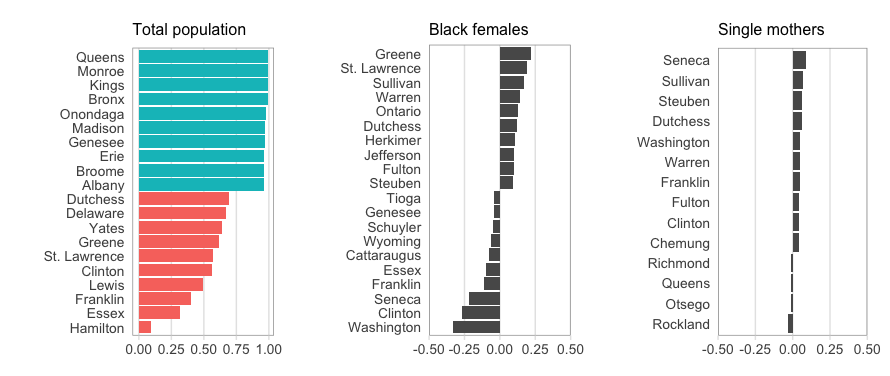
\includegraphics{/Users/johnbrandt/Google Drive/Yale/Semester 1/Environmental Regression/Final/Rplot.png}
\caption{Sample Outputs. \textbf{Left)} Top and bottom 10 counties by
percentage of population within service area. \textbf{Middle)} Top and
bottom 10 counties where black females have more (positive) or less
(negative) access to WIC centers than the general population.
\textbf{Right)} Same as middle, but representing single mothers.}
\end{figure}

\begin{figure}[htbp]
\centering
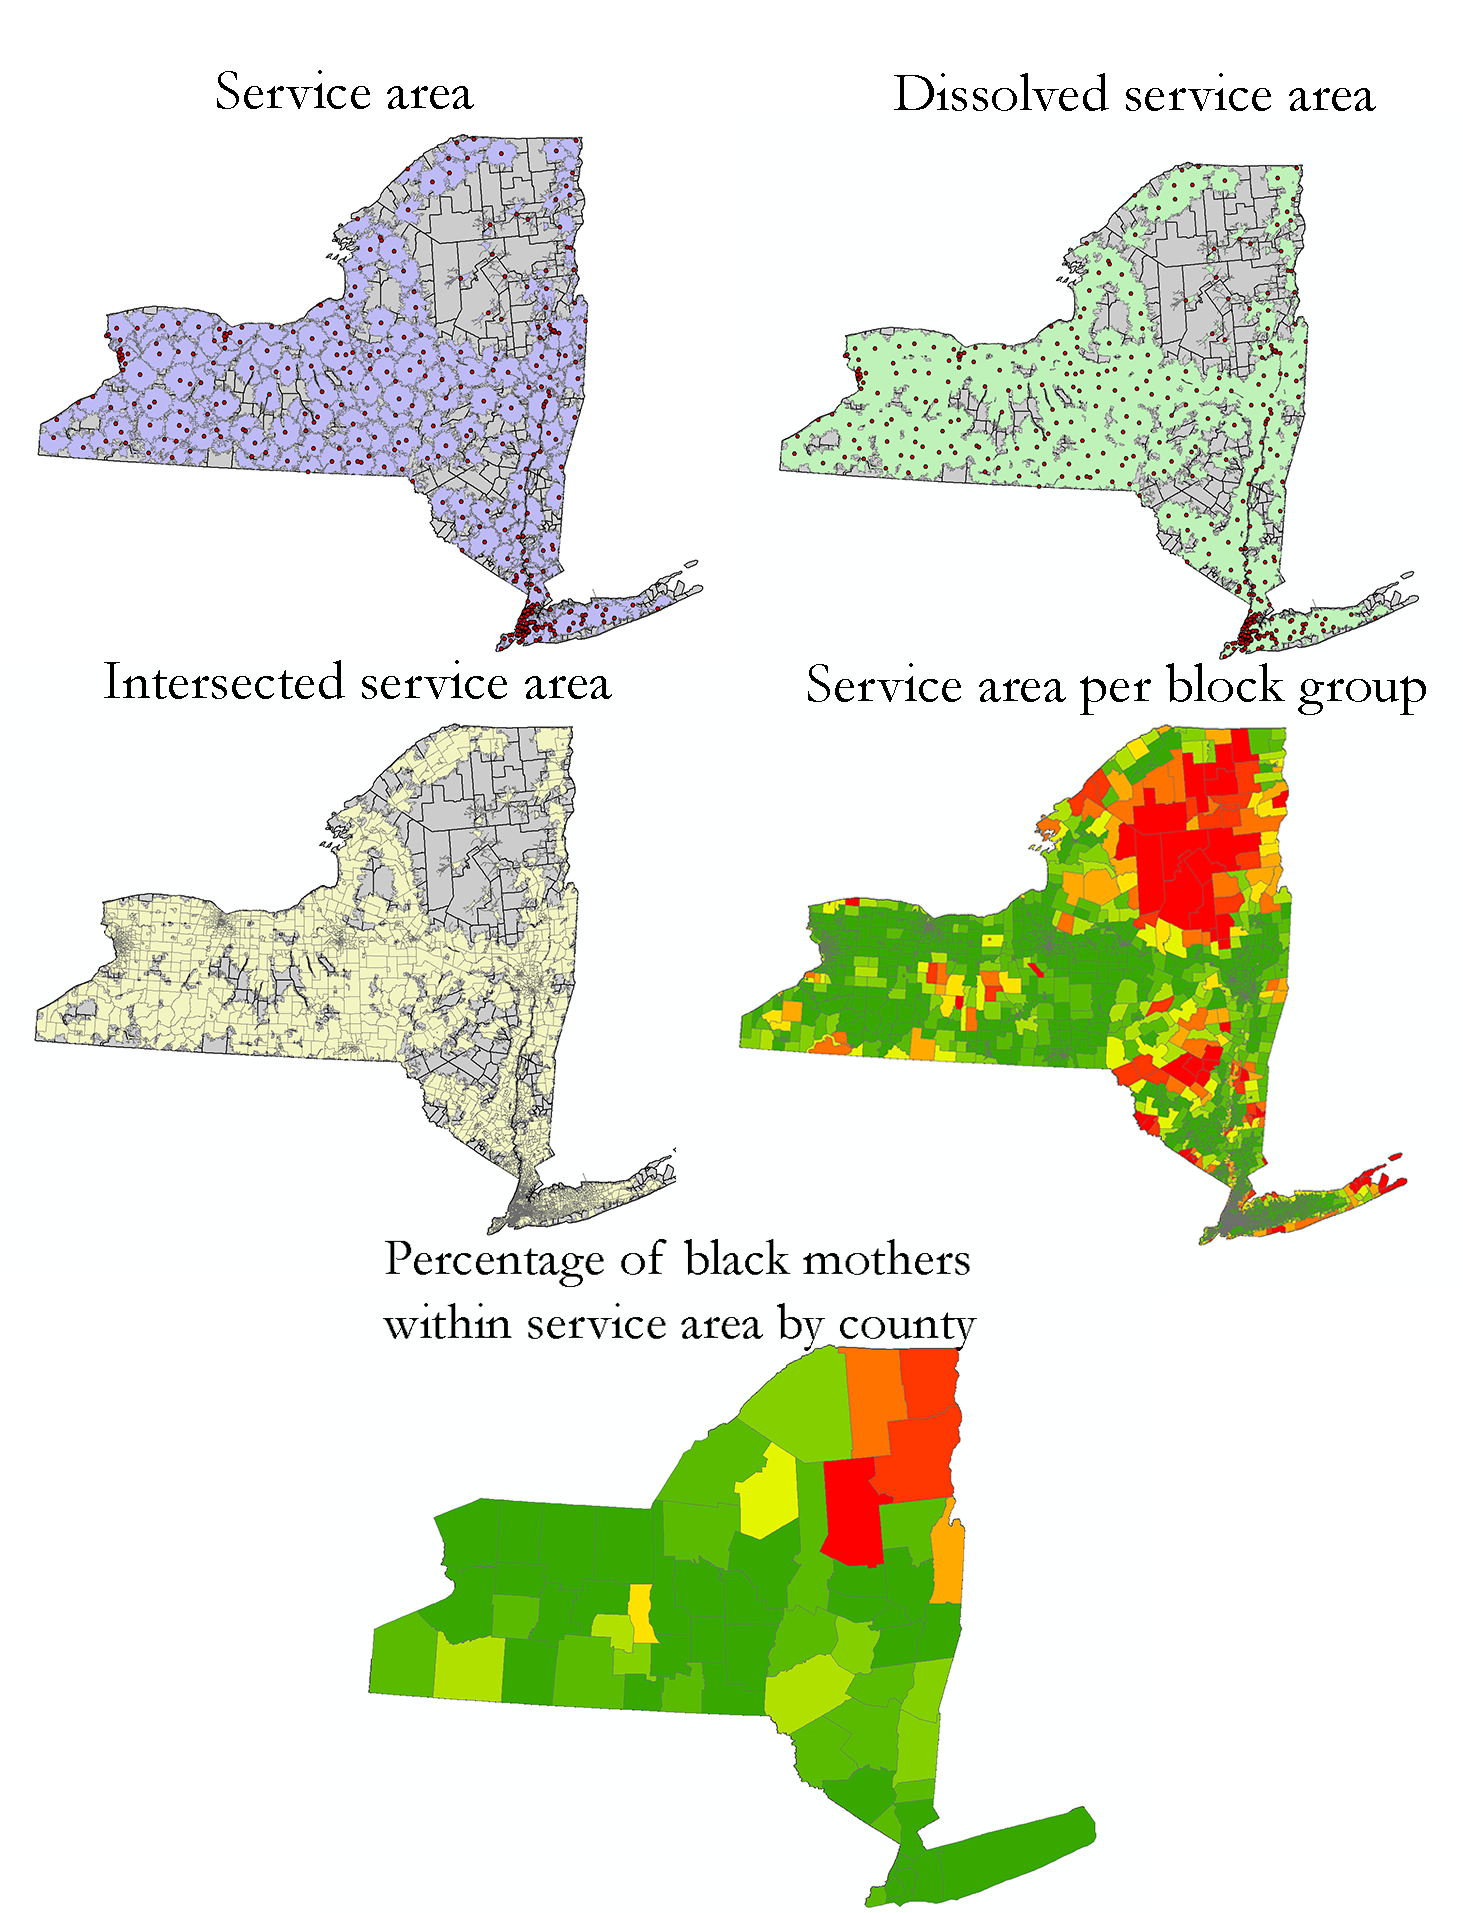
\includegraphics{/Users/johnbrandt/Google Drive/Yale/Semester 1/Environmental Regression/Final/outputs.png}
\caption{Overview of output files}
\end{figure}




\newpage
\singlespacing 
\bibliography{/Users/johnbrandt/Dropbox/master.bib}

\end{document}
